\documentclass[10pt,twocolumn,letterpaper]{article}

\usepackage{iccv}
\usepackage{times}
\usepackage{epsfig}
% \usepackage{graphicx}
\usepackage{amsmath}
\usepackage{amssymb}
\usepackage[activate]{pdfcprot}
\usepackage[usenames,dvipsnames]{xcolor}
\usepackage[color]{changebar}

% Include other packages here, before hyperref.

% for figures and captions
\usepackage{graphicx}
\usepackage{subcaption}
\graphicspath{{figs/}}

% If you comment hyperref and then uncomment it, you should delete
% egpaper.aux before re-running latex.  (Or just hit 'q' on the first latex
% run, let it finish, and you should be clear).
\usepackage[pagebackref=true,breaklinks=true,letterpaper=true,colorlinks,bookmarks=false]{hyperref}

% \iccvfinalcopy % *** Uncomment this line for the final submission

\def\iccvPaperID{****} % *** Enter the ICCV Paper ID here
\def\httilde{\mbox{\tt\raisebox{-.5ex}{\symbol{126}}}}

\cbcolor{Red}
\newcommand{\todo}[1]{\cbstart \textsf{\textbf{\textcolor{Red}{[#1]}}} \cbend{}}
\newcommand{\commentE}[1]{\textsf{\textbf{\textcolor{Green}{Erroll: #1}}}}
\newcommand{\commentA}[1]{\textsf{\textbf{\textcolor{Orange}{Andreas: #1}}}}
\newcommand{\commentT}[1]{\textsf{\textbf{\textcolor{Blue}{Tadas: #1}}}}
\newcommand{\commentY}[1]{\textsf{\textbf{\textcolor{Blue}{Yusuke: #1}}}}

% create a command to set dataset name
\usepackage{xspace}
\newcommand{\dataset}{SynthesEyes\xspace}

% Pages are numbered in submission mode, and unnumbered in camera-ready
\ificcvfinal\pagestyle{empty}\fi
\begin{document}

%%%%%%%%% TITLE
\title{Rendering Photorealistic Training Images for Eye Tracking}

\author{First Author\\
Institution1\\
Institution1 address\\
{\tt\small firstauthor@i1.org}
% For a paper whose authors are all at the same institution,
% omit the following lines up until the closing ``}''.
% Additional authors and addresses can be added with ``\and'',
% just like the second author.
% To save space, use either the email address or home page, not both
\and
Second Author\\
Institution2\\
First line of institution2 address\\
{\tt\small secondauthor@i2.org}
}

\maketitle
%\thispagestyle{empty}

%%%%%%%%% ABSTRACT
\begin{abstract}
   The ABSTRACT is to be in fully-justified italicized text, at the top
   of the left-hand column, below the author and affiliation
   information. Use the word ``Abstract'' as the title, in 12-point
   Times, boldface type, centered relative to the column, initially
   capitalized. The abstract is to be in 10-point, single-spaced type.
   Leave two blank lines after the Abstract, then begin the main text.
   Look at previous ICCV abstracts to get a feel for style and length.
\end{abstract}

%%%%%%%%% BODY TEXT


\section{Introduction}


\section{Related work}

%!TEX root = syntheyes15.tex

\section{Synthetic data generation}

\cite{MIL-STD-1472G} -- cite for range of eye rotation.

\begin{figure}
    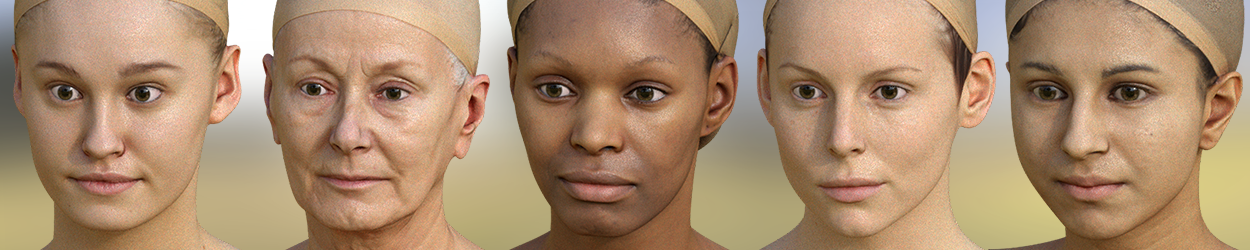
\includegraphics[width=\columnwidth]{participants_f} \par \smallskip
    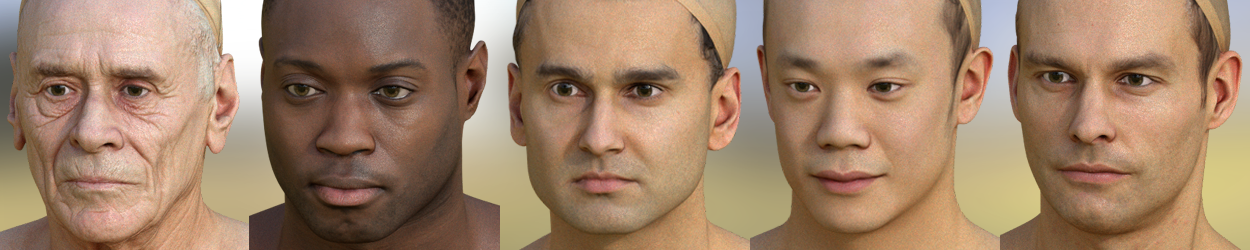
\includegraphics[width=\columnwidth]{participants_m}
    \caption{Our suite of female and male head models for rendering.}
    \label{fig:participants}
\end{figure}

\begin{figure}
    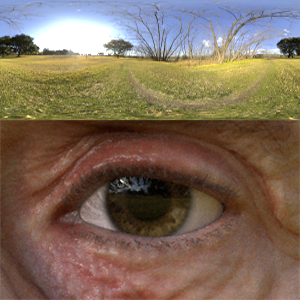
\includegraphics[width=0.24\columnwidth]{fig_env_1} \hfill
    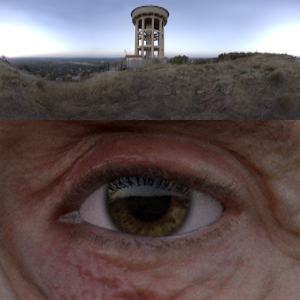
\includegraphics[width=0.24\columnwidth]{fig_env_2} \hfill
    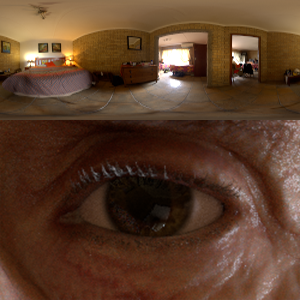
\includegraphics[width=0.24\columnwidth]{fig_env_3} \hfill
    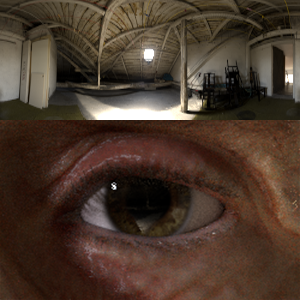
\includegraphics[width=0.24\columnwidth]{fig_env_4}
    \caption{Appearance variation from lighting is modelled with poseable high-dynamic-range environment maps \cite{debevec2002image}.}
    \label{fig:participants}
\end{figure}

\subsection{Eye model}

\begin{figure}
    \centering
    \begin{subfigure}[t]{0.33\columnwidth}
        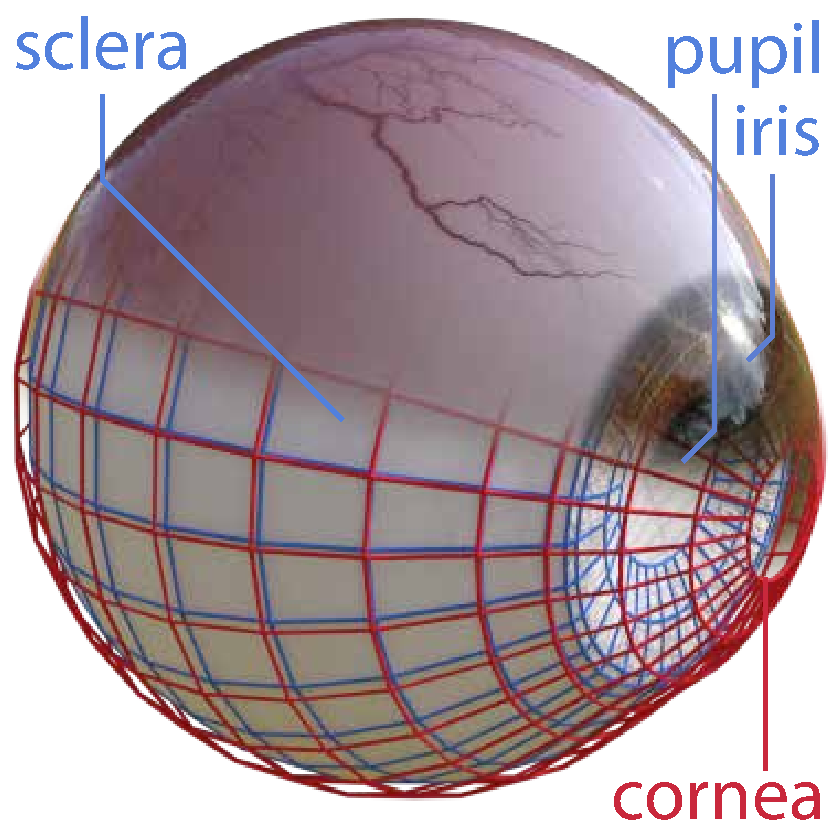
\includegraphics[width=\textwidth]{eye_model}
        \caption{3D eye model}
        \label{fig:3d_eye_model}
    \end{subfigure}%
    \hfill
    \begin{subfigure}[t]{0.65\columnwidth}
        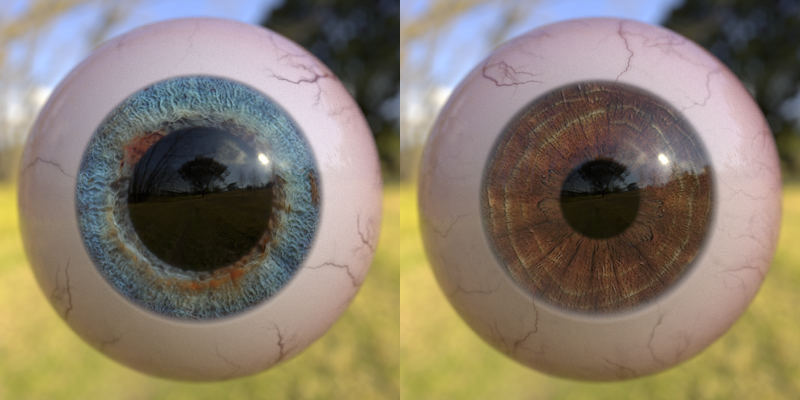
\includegraphics[width=\textwidth]{eye_examples}
        \caption{Pupil dilation and iris color variation}
    \end{subfigure}
    \caption{Our realistic eye model is capable of expressing degrees of variability seen in real life.}
    \label{fig:eye_model}
\end{figure}

Eyeballs are complex organs comprised of multiple layers of tissue, each with different reflectance properties and levels of transparency. Fortunately, as realistic eyes are so important for many areas of CG, there is already a large body of previous work on modelling and rendering eyes \commentE{cite}.

% It is important to accurately model reflections and refractions in the eye as they can lead to specular highlights -- these common eye-region image features are often used by eye-tracking algorithms, or can confound approaches that are not robust.

As shown in \autoref{fig:3d_eye_model}, our eye model consists of two parts.
%
The outer part (red wireframe) approximates the eye's overall shape with two spheres ($r_1\!=\!12\textrm{mm}, r_2\!=\!8\textrm{mm}$ \cite{ruhland2014look}), the latter representing the corneal bulge. To avoid a discontinuous seam between spheres, the meshes were joined and then smoothed. It is transparent, refractive ($n\!=\!1.376$), and partially reflective. The eye's bumpy surface variation is modelled by a displacement map generated with noise functions.
%
The inner part (blue wireframe) is a flattened sphere with Lambertian material. The planar end represents the iris and pupil, and the rest represents the sclera -- the white of the eye.
%
There is a $0.5\textrm{mm}$ gap between the outer and inner parts which accounts for the thickness of the cornea.

Eyes exhibit variations in both shape (pupillary dilation) and texture (iris color and scleral veins). To model shape variation we use \emph{shape keys} -- 

To model how iris color varies between people, we 

Iris color varies between people, and it is important for us to model this.

Previous research on iris-synthesis 

Photo-textures were used for the irises

\subsection{Eye-region model suite}

\subsection{Eyelid motion}

Vertical saccades are always accompanied by eyelid motion \cite{liversedge2011oxford}.
%%!TEX root = syntheyes15.tex

\section{Eye-region specific CLM}

\subsection{Evaluation}

\begin{itemize}
	\item Evaluate eyelid landmark accuracy on LFW and M-PIE data, compare against several state-of-the-art CLM methods
	\item Evaluate eyelid and iris landmarks on annotated MPII data, compare against baseline method: majority vote for iris position
\end{itemize}
%!TEX root = syntheyes15.tex

\section{Experiments}

We evaluated the usefulness of our method on two sample problems, namely eyelid detection and gaze estimation.
\commentA{briefly say something about significance/importance of both problems, more in corresponding subsections}

\subsection{Eyelid Detection}

\commentA{results look pretty good already, I suggest put them in asap so that we can completely draft this subsection. If results improve we can always update later but this way we have something to produce text and refine the story}

\begin{itemize}
    \item Evaluate eyelid landmark accuracy on LFW and M-PIE data, compare against several state-of-the-art CLM methods.
    \item Evaluate eyelid and iris landmarks on hand-annotated MPII data, compare against a baseline method: majority vote for iris position.
\end{itemize}

% show that we only need data from few(er) people and show competitive performance
(Maybe) Plot landmark accuracy on LFW against number of training participants. Show that even with just a few participants (e.g. 4) we get good results for eyelid positions compared to state-of-the-art face trackers.

% eye corner detection
% eye bounding box detection
% eye position detection?
% ^ I think all of these come with what the deformable model gives us

\subsection{Gaze Estimation}

% evaluate eye/gaze/eyelid shapes (fully synthetic) separately from full face appearance (which is a mixture of real and synthetic data)

% person-adaptation, use pre-trained model from synthesised data, then personalise with small amount of user-specific data
% ^ let's leave this as future work! Can put it in the discussion 

% show that we can synthesise specific datasets for specific settings (specific head and gaze ranges, illumination conditions), show that we can competitive performance
We render a targeted dataset that matches MPII's gaze and pose distribution, with added 3D laptop screen emitting light. This shows how we can target specific scenarios like laptop-based gaze estimation, and render a suitable dataset within a day rather than take 3 months of data collection.

% train on synthesised images and show competitive performance on MPIIgaze with real images
% show better performance than UT dataset
Using Xucong's CNN sytem, we train on targeted version of \dataset, test on MPII. Show results are better than training on UT and testing on MPII. This shows that the range of lighting in \dataset is important for better results.

% does photorealistic data really help/is it necessary? either reduce quality and see how it affects performance, or compare model with and without shape variations
% ^ I am not really sure how to do this well... Because we'd also have to have a measure of "how photorealistic" something is. Swapping the eyeball for a simpler model, e.g. sphere might not really have that much of an effect on "photorealism" for many eye-poses. Changing the shaders, e.g. pretending the skin is Lambertian (diffuse) might?



\section{Conclusion}



{\small
\bibliographystyle{ieee}
\bibliography{bib}
}

\end{document}
